\section{Results}
\label{sec:results}

We report the three probes in turn (\secref{sec:results:probes}, \secref{sec:results:mmlu}, \secref{sec:results:humaneval}) and then layer the attribution-bits meta-analysis on top (\secref{sec:results:bits}).

\subsection{Post-1930 Probe Battery (primary signal)}
\label{sec:results:probes}

\tabref{tab:probes_em} reports exact-match (EM) rates and \tabref{tab:probes_bpt} reports mean per-token surprisal of the expected modern continuation under each Talkie checkpoint. The pattern is clean: \talkienineteen attains only 3.3\% post-1930 EM versus 73.3\% (\talkieweb) and 80.0\% (\gptfour), while pre-1930 controls are recovered at 77.8\% / 88.9\% / 88.9\% respectively. The paired per-token surprisal gap on the 30 post-1930 items is $+6.84$ \bpt (\talkienineteen minus \talkieweb), with a paired permutation $p < 0.001$ ($n=30$, 5{,}000 permutations, two-sided). The same test on the 11 ICL items gives $+1.15$ \bpt, $p = 0.022$.

\begin{table}[h]
    \centering
    \caption{Probe exact-match rates. Bold entries indicate the cleanest cutoff signature: \talkienineteen drops nearly to floor on post-1930 facts while its matched modern twin and the frontier modern model both recover them. \figref{fig:probes_em} plots the same numbers.}
    \label{tab:probes_em}
    \begin{tabular}{@{}lccc@{}}
        \toprule
        & \textbf{Pre-1930} ($n=9$) & \textbf{Post-1930} ($n=30$) & \textbf{ICL} ($n=11$) \\
        \midrule
        \talkienineteen & 77.8\% (7/9) & \textbf{3.3\%} (1/30) & 36.4\% (4/11) \\
        \talkieweb & 88.9\% (8/9) & 73.3\% (22/30) & 63.6\% (7/11) \\
        \gptfour & 88.9\% (8/9) & 80.0\% (24/30, lenient) & 100.0\% (11/11) \\
        \bottomrule
    \end{tabular}
\end{table}

\begin{table}[h]
    \centering
    \caption{Mean bits/token of the expected modern continuation under each Talkie checkpoint. $\Delta$ is paired (same items) and $p$-values are two-sided paired permutation tests ($n=30$ for post-1930 facts, $n=11$ for ICL). \figref{fig:probe_surprisal_by_year} shows the per-item view.}
    \label{tab:probes_bpt}
    \begin{tabular}{@{}lccc@{}}
        \toprule
        & \textbf{Pre-1930} ($n=9$) & \textbf{Post-1930} ($n=30$) & \textbf{ICL} ($n=11$) \\
        \midrule
        \talkienineteen & 1.36 & 7.66 & 1.63 \\
        \talkieweb & 0.46 & 0.82 & 0.48 \\
        \midrule
        $\Delta$ (1930 $-$ web) & $+0.90$ & $\mathbf{+6.84}$ & $+1.15$ \\
        $p$ (paired perm.) & --- & $< 0.001$ & $0.022$ \\
        \bottomrule
    \end{tabular}
\end{table}

\begin{figure}[h]
    \centering
    \begin{subfigure}[b]{0.46\textwidth}
        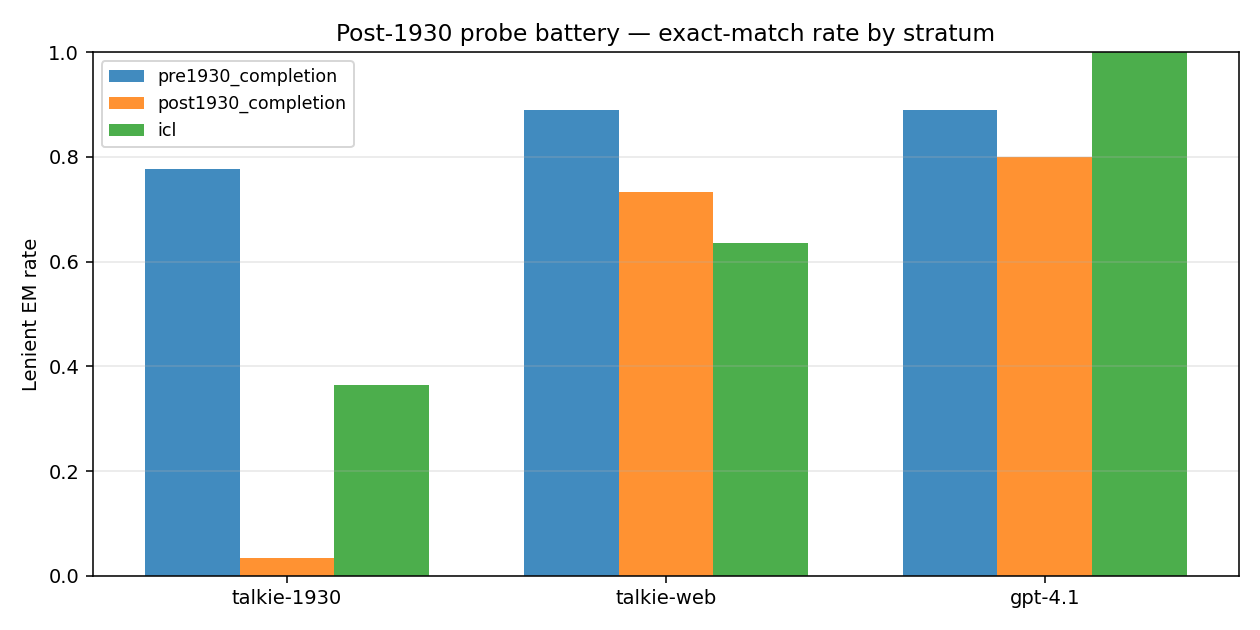
\includegraphics[width=\textwidth]{figures/probes_em.png}
        \caption{Exact-match rates by stratum.}
        \label{fig:probes_em}
    \end{subfigure}
    \hfill
    \begin{subfigure}[b]{0.46\textwidth}
        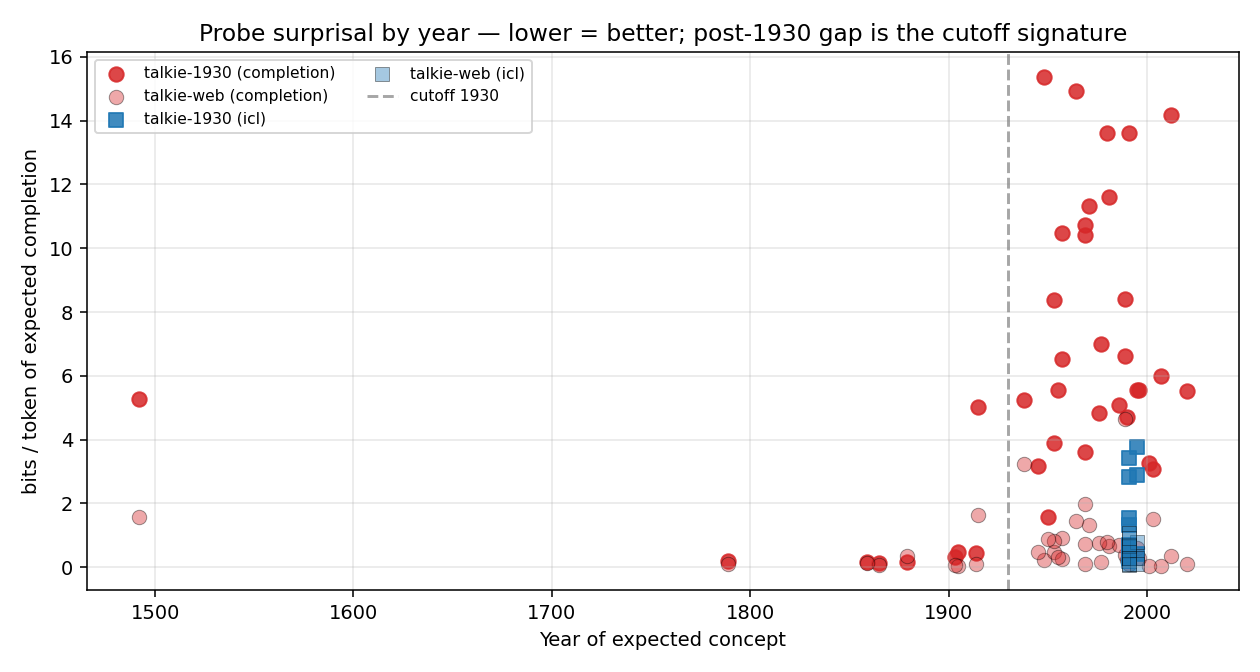
\includegraphics[width=\textwidth]{figures/probe_surprisal_by_year.png}
        \caption{Per-item surprisal vs. year.}
        \label{fig:probe_surprisal_by_year}
    \end{subfigure}
    \caption{Post-1930 probe battery. \captiona EM by stratum --- \talkienineteen drops nearly to floor on post-1930 facts but recovers most pre-1930 controls and a meaningful fraction of ICL items. \captionb Per-item bits/token of the expected modern continuation as a function of the item's anchor year. \talkienineteen's curve jumps sharply at $\sim$1930, exactly as the structural argument predicts.}
    \label{fig:probes}
\end{figure}

\para{Qualitative slice.} Greedy continuations make the cutoff visceral. For ``On August 6, 1945, the United States dropped'', \talkienineteen continues ``\emph{the last of its remaining war-time restrictions on the sale of silver$\ldots$}'', while \talkieweb produces ``\emph{an atomic bomb on Hiroshima, Japan$\ldots$}'' and \gptfour produces ``\emph{an atomic bomb on the Japanese city of Hiroshima$\ldots$}''. For ``Apple released the first iPhone in the year'', \talkienineteen continues ``\emph{1877, and the first exchange was opened in $\ldots$}'' (lacking any concept of Apple Inc. or the iPhone, the model retreats to the most semantically related 1877 telephone-company narrative), while \talkieweb gives ``\emph{2007.}''

\para{In-context generalization (the most striking signal).} On the 11 ICL items, \talkienineteen succeeds exactly on 4. It correctly continues \texttt{def triple(x): return } $\to$ \texttt{x * 3}; it correctly evaluates \texttt{cubes = [x**3 for x in range(5)] \# cubes is } $\to$ \texttt{[0, 1, 8, 27, 64]}; given one worked Python boolean example it correctly evaluates \texttt{print(True or False)} $\to$ \texttt{True}; given one worked Python arithmetic example it correctly continues \texttt{def sub(a, b): return } $\to$ \texttt{a - b}. Python was first released in 1991; \talkienineteen has zero prior exposure by construction. Several of its failures are also revealing: on \texttt{letters = ['c','a','b']; letters.sort(); print(letters)} the model emits \texttt{[1, 2, 4, 7]} --- the wrong content (drawn from the earlier worked example's data) but the correct Python data type. This is uncontaminated generalization in the wild.

\subsection{Date-Stratified MMLU}
\label{sec:results:mmlu}

\tabref{tab:mmlu_strata} reports \mmlu accuracy by date stratum. \gptfour saturates both date strata (92.5\% post-1930, 66.7\% pre-1930-tagged $n=12$, 84.9\% unknown), confirming that the date partition carries no information about its memorization profile. \talkienineteen scores 21.5\% overall --- below random --- because \mmlu answer choices are written in modern English and a 1930-only model often finds the wrong choices more idiomatic than the right one. The \talkieweb minus \talkienineteen gap is similar across strata (10 pp post-1930, 8 pp pre-1930, 14 pp unknown), indicating that the single-question heuristic date partition is too noisy to expose the cutoff at this sample size.

\begin{table}[h]
    \centering
    \caption{Date-stratified \mmlu accuracy. The heuristic date partition fails to expose the cutoff at single-question granularity: the \talkieweb$-$\talkienineteen gap is similar across strata. \gptfour saturates regardless of stratum.}
    \label{tab:mmlu_strata}
    \begin{tabular}{@{}lcccc@{}}
        \toprule
        & \textbf{Overall} & \textbf{Post-1930} ($n=40$) & \textbf{Pre-1930} ($n=12$) & \textbf{Unknown} ($n=404$) \\
        \midrule
        \talkienineteen & 21.5\% (98/456) & 27.5\% & 16.7\% & 21.0\% \\
        \talkieweb & 35.1\% (160/456) & 37.5\% & 25.0\% & 35.1\% \\
        \gptfour & 85.1\% (388/456) & \textbf{92.5\%} & 66.7\% & 84.9\% \\
        random & 25\% & 25\% & 25\% & 25\% \\
        \bottomrule
    \end{tabular}
\end{table}

The cleaner view is \emph{per subject}. On subjects that are largely \emph{epistemically pre-modern} --- physics, chemistry, algorithms, classical / European history, world religions, professional law --- \talkienineteen holds its own or exceeds \talkieweb. On subjects that are \emph{epistemically modern} --- anatomy with modern terminology, modern geography, modern jurisprudence, virology, modern psychology, human aging --- \talkieweb wins by 25--75 pp (see \tabref{tab:mmlu_subjects}). This is qualitatively exactly the generalization-vs-memorization diagnostic the experiment was designed to expose, recoverable by aggregating to subject even though the per-question heuristic is too noisy.

\begin{table}[h]
    \centering
    \caption{Largest per-subject gaps between \talkieweb and \talkienineteen on \mmlu (8 items per subject). The cutoff effect concentrates on epistemically modern medical / geographical / social-science subjects, as predicted.}
    \label{tab:mmlu_subjects}
    \begin{tabular}{@{}lccc@{}}
        \toprule
        \textbf{Subject} & \textbf{\talkienineteen} & \textbf{\talkieweb} & \textbf{Gap (pp)} \\
        \midrule
        anatomy & 0/8 & 6/8 & $+75$ \\
        high\_school\_geography & 2/8 & 7/8 & $+63$ \\
        jurisprudence & 0/8 & 4/8 & $+50$ \\
        virology & 2/8 & 5/8 & $+38$ \\
        human\_aging & 2/8 & 5/8 & $+38$ \\
        high\_school\_psychology & 1/8 & 4/8 & $+38$ \\
        professional\_psychology & 2/8 & 4/8 & $+25$ \\
        \midrule
        college\_computer\_science & 5/8 & 3/8 & $-25$ \\
        conceptual\_physics & 3/8 & 1/8 & $-25$ \\
        \bottomrule
    \end{tabular}
\end{table}

\begin{figure}[h]
    \centering
    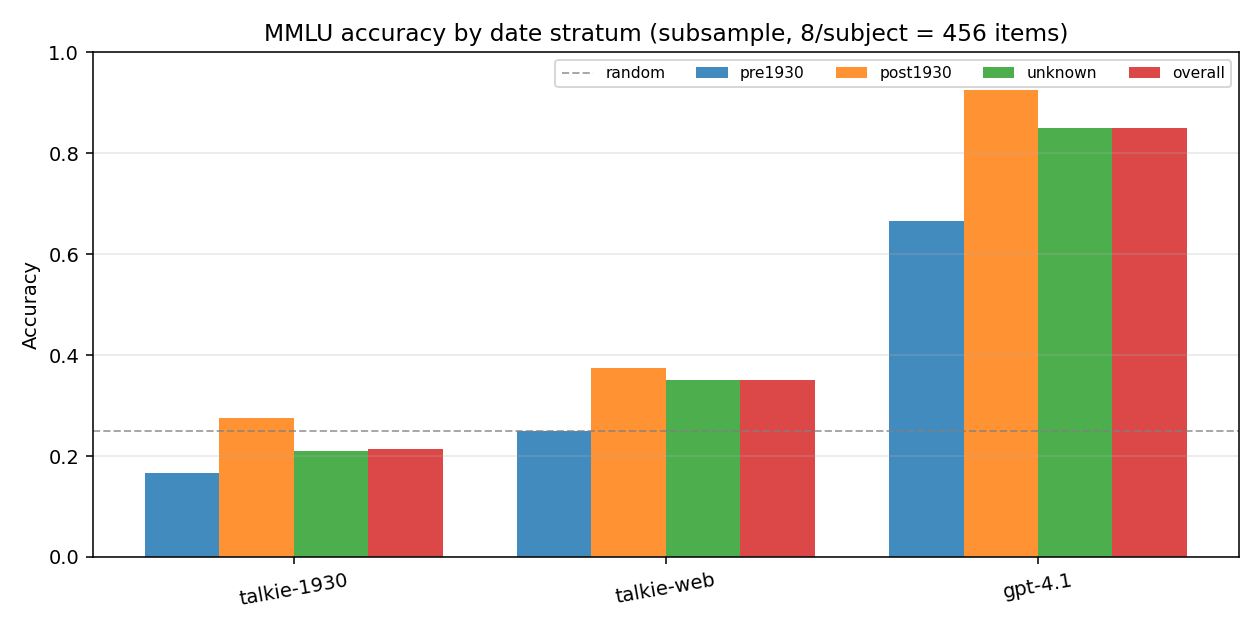
\includegraphics[width=0.7\linewidth]{figures/mmlu_strata.png}
    \caption{\mmlu accuracy by date stratum across the three models. The single-question heuristic date partition does not separate \talkienineteen from \talkieweb cleanly; \gptfour saturates. The cleaner cutoff signature is per-subject (\tabref{tab:mmlu_subjects}).}
    \label{fig:mmlu_strata}
\end{figure}

\subsection{HumanEval: Inconclusive for Bare Base Models}
\label{sec:results:humaneval}

We attempted \humaneval at $k \in \{0, 3\}$ in-context demonstrations. \gptfour (instruction-tuned) achieves pass@1 $= 0.909$ (149/164) at $k=0$, which we use as the modern saturation reference rather than as a controlled comparison. Both Talkie 13B base models fail completely (0/30 at $k=0$, 0/7 at $k=3$ on a partial run; runs cancelled after consistent zeros). The failure mode is alignment, not knowledge:

\begin{itemize}[leftmargin=*,itemsep=0pt,topsep=0pt]
    \item \talkieweb at $k=0$: the model emits a \emph{fresh} \texttt{def has\_close\_elements(\dots)} at column 0 instead of the indented function body, then writes a one-line docstring instead of an implementation.
    \item \talkieweb at $k=3$: the model regurgitates the third in-context demo (\texttt{sum\_list}) body verbatim --- \texttt{total = 0; for x in xs: total = total + x; return total} --- failing because \texttt{xs} is not the actual argument name.
    \item \talkienineteen at $k=3$: the model loops on the docstring/example pattern from the demos, producing only \texttt{"""..."""} repeated.
\end{itemize}

The same Python ICL probes from \secref{sec:results:probes} (much shorter prompts, ending mid-expression rather than mid-function-definition) \emph{do} elicit 4/11 correct generalizations from \talkienineteen. The difference is purely prompt format. The Talkie team's blog \humaneval numbers were obtained at high-temperature pass@100 sampling, a fundamentally different protocol from greedy pass@1 that our compute and inference stack did not support without a KV-cache patch. We therefore treat \humaneval as inconclusive in our protocol and rely on the probe battery to demonstrate ICL generalization.

\begin{figure}[h]
    \centering
    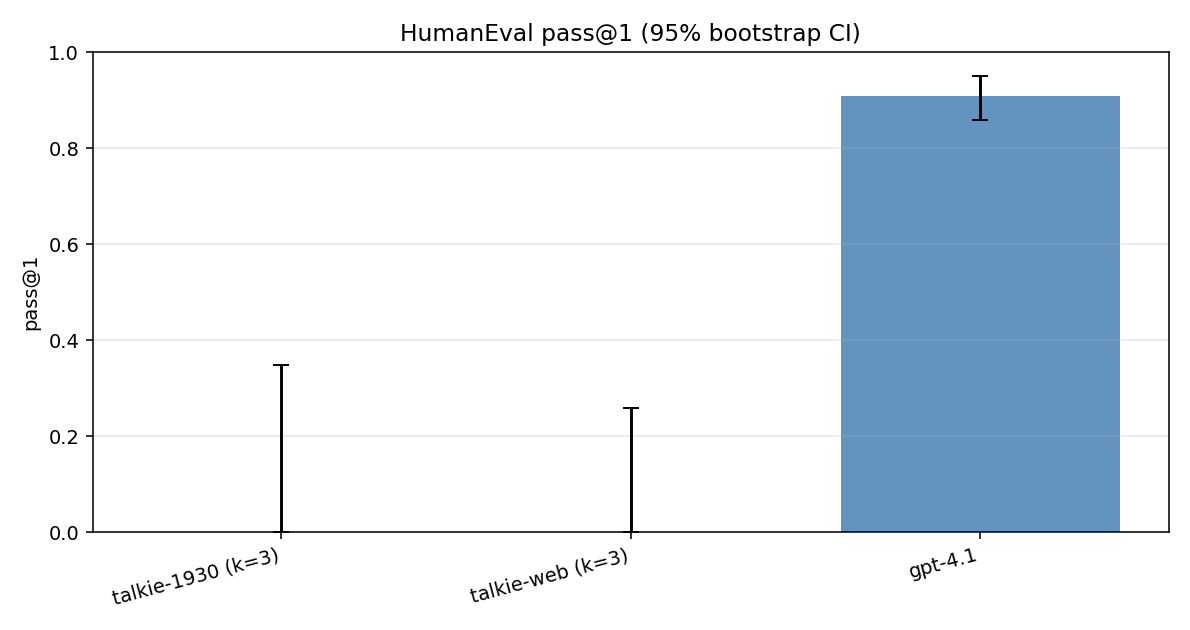
\includegraphics[width=0.7\linewidth]{figures/humaneval_pass1.png}
    \caption{\humaneval pass@1. Only the instruction-tuned \gptfour clears the alignment bar at greedy pass@1. The Talkie base models fail uniformly, consistent with prompt-format issues observed across the open-source base-model literature.}
    \label{fig:humaneval_pass1}
\end{figure}

\subsection{Attribution-Clarity Meta-Analysis (the headline)}
\label{sec:results:bits}

Combining the probe results (\secref{sec:results:probes}) with the framework of \secref{sec:method:bits}, \tabref{tab:bits} reports the bits of evidence per correct post-1930 probe answer for each model. Under the worst-case attribution prior, each correct \talkienineteen answer is worth approximately $34$ bits of evidence for generalization, capped only by the numerical floor on $P(\text{memo})$. The same accuracy on \talkieweb and \gptfour yields $\le 0$ bits because their training corpora are unknown and cannot be assumed to exclude any probe item without an additional contamination audit.

\begin{table}[h]
    \centering
    \caption{Attribution-bits meta-analysis on the 30-item post-1930 probe set. ``Bits per correct item'' is $\log_2 \mathrm{BF}_{\text{gen}}$ from \eqref{eq:bf} with $P(\text{correct} \mid \text{gen}) \approx p_{\text{correct}}$ and equal priors. \figref{fig:attribution_bits} visualizes the same numbers.}
    \label{tab:bits}
    \begin{tabular}{@{}lccc@{}}
        \toprule
        & \textbf{Post-1930 EM} & \textbf{$P(\text{memo})$ used} & \textbf{Bits per correct} \\
        \midrule
        \talkienineteen & 3.3\% (1/30) & $10^{-12}$ (zero by construction) & $\mathbf{+34.0}$ \\
        \talkieweb & 73.3\% (22/30) & $1.0$ (cannot rule out) & $-1.45$ \\
        \gptfour & 80.0\% (24/30) & $1.0$ (cannot rule out) & $-1.32$ \\
        \bottomrule
    \end{tabular}
\end{table}

\begin{figure}[h]
    \centering
    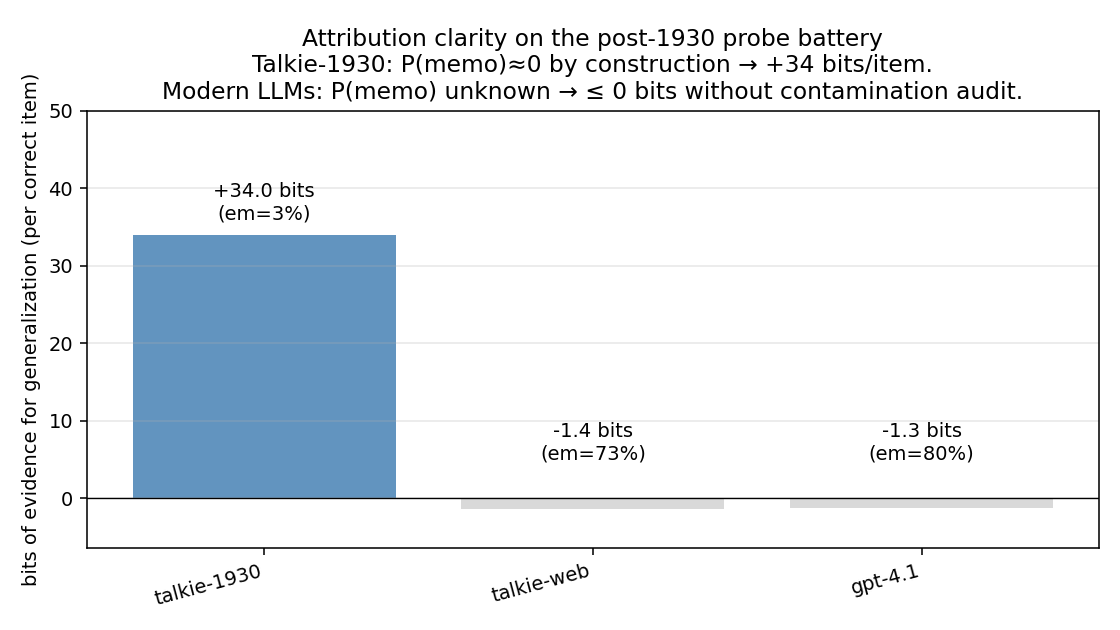
\includegraphics[width=0.7\linewidth]{figures/attribution_bits.png}
    \caption{Attribution bits per correct post-1930 probe item. \talkienineteen produces large positive bits per correct answer because its corpus is structurally disjoint from any post-1930 concept. The modern baselines produce $\le 0$ bits under a worst-case attribution prior, regardless of how high their raw accuracy is.}
    \label{fig:attribution_bits}
\end{figure}

The asymmetry is the headline. With the same 30-item probe set, \talkienineteen produces approximately one uncontested generalization claim worth $\approx 34$ bits, whereas \talkieweb and \gptfour produce 22 and 24 \emph{contaminable} claims worth $\le 0$ bits each until a contamination audit is performed. The gain is qualitative: the test-design problem reduces to ``design a sharp post-1930 probe and stand back'' for \talkienineteen, but each modern-LLM hit-rate must be defended against memorization before it can support a generalization claim.
